
\subsection{ExperimentalData}
\label{sec:ExperimentalData}


\begin{figure}[ht]
\begin{center}
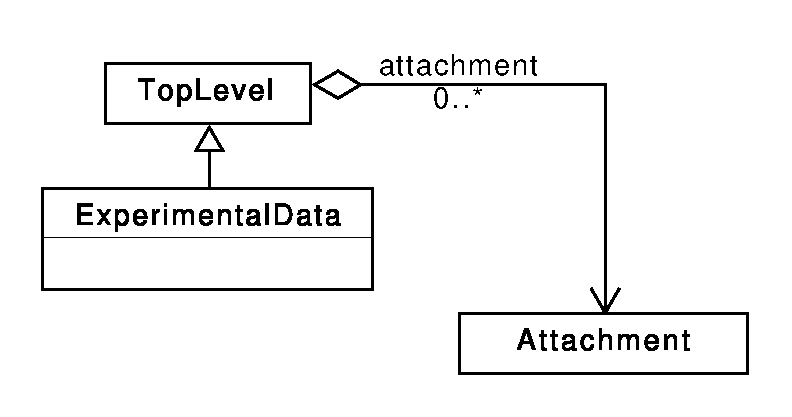
\includegraphics[scale=0.6]{uml/experimental_data}
\caption[]{Diagram of the \sbol{ExperimentalData} class and its associated properties.}
\label{uml:experimental_data}
\end{center}
\end{figure}

The purpose of the \sbol{ExperimentalData} class is to aggregate links to experimental data files. An \sbol{ExperimentalData} is typically associated with a single sample, lab instrument, or experimental condition and can be used to describe the output of the test phase of a design-build-test-learn workflow. For an example of the latter, see \ref{images:design-build-test-learn}.

As shown in \ref{uml:experimental_data}, the \sbol{ExperimentalData} class aggregates links to experimental data files using the OPTIONAL \sbol{hasAttachment} property that it inherits from the \sbol{TopLevel} class.
